\documentclass{article}

% if you need to pass options to natbib, use, e.g.:
% \PassOptionsToPackage{numbers, compress}{natbib}
% before loading nips_2016
%
% to avoid loading the natbib package, add option nonatbib:
\usepackage[square,numbers]{natbib}

% to compile a camera-ready version, add the [final] option, e.g.:
\usepackage[final]{nips_2016}

\usepackage[utf8]{inputenc} % allow utf-8 input
\usepackage[T1]{fontenc}    % use 8-bit T1 fonts
\usepackage{hyperref}       % hyperlinks
\usepackage{url}            % simple URL typesetting
\usepackage{booktabs}       % professional-quality tables
\usepackage{amsmath}
\usepackage{amsfonts}       % blackboard math symbols
\usepackage{nicefrac}       % compact symbols for 1/2, etc.
\usepackage{microtype}      % microtypography
\usepackage{graphicx}
\usepackage{enumerate}
\title{10-715 Project Final Report \\
Multitask Learning for Semantic Acoustical Embedding  
}

% The \author macro works with any number of authors. There are two
% commands used to separate the names and addresses of multiple
% authors: \And and \AND.
% Using \And between authors leaves it to LaTeX to determine where to
% break the lines. Using \AND forces a line break at that point. So,
% if LaTeX puts 3 of 4 authors names on the first line, and the last
% on the second line, try using \AND instead of \And before the third
% author name.

\author{
  Daniel Clothiaux\\
  \texttt{dclothia@cs.cmu.edu}
  \And
  Qinlan Shen\\
  \texttt{qinlans@cs.cmu.edu}
  \And
  Wenbo Zhao\\
  \texttt{wzhao1@andrew.cmu.edu}
}

\begin{document}

\maketitle

\begin{abstract}
Word embeddings have been widely used in various text processing tasks as a way to encode information about its semantic and syntactic properties. Multitask learning can be used when training word embeddings to both generate shared representations for related tasks and learn properties from multiple sources of information. In speech processing, vector acoustic embeddings have recently emerged as an alternative to phonetic unit-based speech representation. While these embeddings are effective in mapping similar sounding words to a similar space, they do not capture other properties of the utterance, such as the semantics of the word being said or information about the speaker of an utterance. We propose a multitask learning framework for semantic acoustic embeddings that encode both phonetic and semantic information of an utterance. In addition to what word is being said and its semantics, we attempt to incorporate other properties found in the speech signal such as gender, age, dialect, and speaker identity, in our speech embeddings.
\end{abstract}

\section{Introduction}
Many tasks in natural language processing rely on vector embeddings to provide a mathematical representation for a language unit, such as a word, a morpheme, or a sentence. These representations encode information about the properties of a word in a given context, so that units that have similar properties are close together in the mapped space. This provides more information than simply treating a word as a discrete or atomic unit. While word embeddings are vastly popular in text-based natural language processing, acoustic vector embeddings for speech applications have only recently grown in popularity \citep{bengio2014word,kamper2016deep,ghannay2016evaluation}. These acoustic embeddings attempt to project speech utterances that sound similar to fixed-dimension vectors so that they are close by some distance metric. The use of speech embeddings in place of phonetic-unit based speech recognition has led to improvements in automatic speech recognition \citep{bengio2014word} and word discrimination \citep{kamper2016deep}.  However, speech embeddings currently only capture the acoustic properties of what is being said.  For downstream tasks that also rely on the meaning of what is being said, additional word embeddings would be necessary to capture the meaning of an utterance.  Additionally, speech utterances contain more information than just the spoken words -- a speaker's identity, gender, age, or emotion can also be extracted from the speech signal.  Thus, our goal is to create generalized speech embeddings that consider both semantic and acoustic similarities between utterances. We propose a semantic acoustic embedding framework that encodes the acoustic and semantic information of speech utterances as vectors using multitask learning. These mixed embeddings would ideally improve performance on downstream speech-related tasks \citep{audhkhasi2016semantic} by incorporating information about the speaker and the semantics of what is being said.

\subsection{Contributions of this Paper}
The contributions of this paper are three-folded. First, we propose a semantic acoustic embedding that encodes the acoustic and semantic information of speech utterances into vector embeddings. This takes into consideration both the acoustical and semantic information of speech signals, and aids the related downstream tasks with compact representations. Second, we propose a multitask learning framework that uses the embeddings to do task-specific predictions. The seven tasks that we used in our multitask learning architecture are
\begin{enumerate}[(1)]
	\item Word recognition: given an acoustic speech segment, predict the word that was uttered in the segment.
	\item Word semantic prediction: given an acoustic speech segment, minimize the distance between the prediction and the pretrained embedding of the word that was uttered.
	\item Gender prediction: given an acoustic speech segment, predict the gender of the speaker.
	\item Speaker identification: given an acoustic speech segment, predict which speaker is speaking.
	\item Age prediction: given an acoustic speech segment, predict the age range of the speaker.
    \item Education prediction: given an acoustic speech segment, predict the education level of the speaker.
	\item Dialect prediction: given an acoustic speech segment, predict the dialect of the speaker.
\end{enumerate}
Third, we empirically show that with our proposed architecture, we are able to predict the each individual task with high accuracy, but have errors when predicting multitasks because these tasks are not related closely enough to give generative shared speech embeddings. Thus, we need a more robust technique than basic multitask learning in order to construct embeddings that contain properties from all of these tasks.

\section{Related Work}
In speech recognition, input speech frames are usually converted to their Mel-Scale Frequency Cepstral Coefficients (MFCC) \citep{ittichaichareon2012speech} representations. A Hidden Markov Model (HMM) is then constructed with its states representing the phonetic units in the utterances \citep{bengio2014word}. The goal is to find the optimal parameters for the HMM such that the state transitions match best with the utterances. Conventional approaches treat each state as a Gaussian mixture models (GMM) distribution \citep{saini2013automatic}. While effective, GMM tends to represent the data with a large number of parameters, whereas the true underlying structure is of a much lower dimension \citep{hinton2012deep}. Literature shows that estimating the \emph{posterior} probabilities of the HMM states using deep neural networks outperforms GMM in many benchmarks \citep{hinton2012deep}. Further, in tasks like speaker verification, speech segmentation, and emotion recognition, dimension reduction techniques such as joint factor analysis and i-vectors can characterize the speaker and channel variability \citep{kenny2014joint,garimella2015robust,chen2011applying,chen2013emotional,andrew2014improve,karanasou2014adaptation}.

As an alternative to phonetic unit representation, acoustic vector embeddings have grown increasingly popular \citep{bengio2014word,kamper2016deep,ghannay2016evaluation}. The primary goal of speech embedding is to map similar acoustic segments to similar spaces. Bengio et al. \citep{bengio2014word} create speech embeddings by using a convolutional neural network to learn a mapping between acoustic sequences and word probabilities. They then use triple ranking loss to simultaneously push the embeddings towards the correct word and away from a randomly selected incorrect word. Kamper et al. \citep{kamper2016deep} train their speech embeddings on a word discrimination task using a convolutional neural network over word pairs. Ghannay et al. \citep{ghannay2016evaluation} propose two methods to intrinsically evaluate speech embeddings by comparing them with orthographic representations.

Multitask learning has been applied to many natural language processing problems using different sets of tasks. Collobert et al. \citep{collobert2008unified} train word embeddings against a wide range of NLP tasks, such as language modeling, part of speech tagging, and named entity recognition. These tasks share a deep architecture with a feed-forward layer on top of a convolutional layer. The output of the shared architecture is then fed into separate task-specific components. Liu et al. \citep{liu2015representation} base their model on a similar architecture, building a shared representation using three feed-forward layers to represent bag-of-words, letter n-grams, and semantics, respectively.  This shared representation is then fed into the task-specific components (in this case, query classification and web search). While both of these papers train shared lower layers by propagating the errors from the task-specific higher layers, Sogaard et al. \citep{sogaard2016deep} associates each layer of the network with a different task and supervise each task from its corresponding layer. Luong et al. \citep{luong2015multi} propose several architectures for multitask sequence-to-sequence learning using multiple encoders and/or decoders.

\section{Methods}
In this section, we mathematically formulate our problem, and present the multitask learning framework to solve the problem.
\subsection{Problem Formulation}
Consider a sequence of $N$ word features
$\mathbf{W} = \{ \mathbf{w}_1, \mathbf{w}_2, \ldots, \mathbf{w}_N \} \subseteq \mathcal{W}$, where each feature $\mathbf{w}_i \in \mathbb{R}^{F \times D}$, $i=1,\ldots,N$, and the symbol $F$ and $D$ denote the number of frames and the dimension of each frame in each word feature respectively. The corresponding labels for $\mathbf{W}$ are $\mathbf{y} = \{\mathbf{y}^t: t \in \mathcal{T} \}\subseteq \mathcal{L}$, where $\mathcal{T}$ is the task space and $\mathcal{L}$ is the complete label space. Our goal is to find the optimal mapping $\mathcal{F}: \mathcal{W} \to \mathcal{L}$ such that
\begin{equation}
f^t = \mathrm{argmin}_{f^t \in \mathcal{F}, t \in \mathcal{T}} \mathcal{R}(f^t(\mathbf{W}), \mathbf{y}^t),
\end{equation}
where $\mathcal{R}$ is the risk function that evaluates the risk for $f$. For each specific task $t \in \mathcal{T}$, the corresponding objectives are

\begin{align}
f^t = \left\{\begin{matrix}
& \mathrm{argmin}_{f^t \in \mathcal{F}}\, -\log{f^t(\mathbf{W},\mathbf{y}^t)} \\
& t \in \{\textup{speech recognition, speaker identification, gender, education, dialect}\}, \\
& \mathrm{argmin}_{f^t \in \mathcal{F}}\, \|f^t(\mathbf{W}) - \mathbf{y}^t\|_2 \\
& t \in \{\textup{semantic similarity, age}\},
\end{matrix}
\right.
\end{align}
where we minimize the negative log-likelihood $-\log{\prod_{i}^{N}{P(\mathbf{y}_i^t|\mathbf{w}_i)}}$ for the classification-based tasks (speech recognition, speaker identification, gender, education, and dialect) and minimize the mean square error for the regression-based tasks (semantic similarity and age). We propose a multitask learning framework that finds the optimal $f$ for each task. The framework constructs a neural network containing convolutional layers, a shared embedding layer, and task-specific feedforward layers, and learns and optimizes the mapping from the word feature space $\mathcal{W}$ to label space $\mathcal{L}$ by gradient backpropagation.

\subsection{Multitask Learning Framework for Acoustical Embedding}
\begin{figure}[h!]
\centering
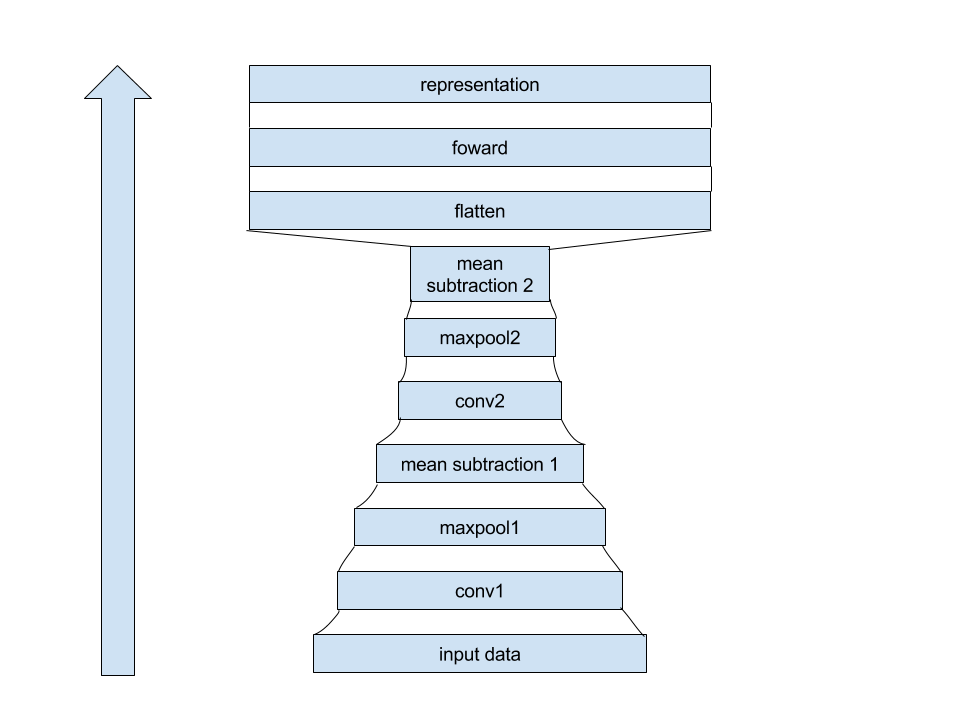
\includegraphics[scale=.2]{convnet_layers.png}
\caption{The convolutional layers up to the representation}
\label{fig:shared}
\end{figure}
We implement a convolutional neural network (CNN) framework for multitask learning.  Input data instances are run through two convolutional layers with relu nonlinearity, each followed by a max pooling layer and a mean subtraction layer. A maxpool layer has a fixed range and stride and returns the maximum value among the elements in its range. A mean subtraction layer calculates the mean of the previous layer within a sliding window, then subtracts it from the elements of the previous layer in the window.  These two operations are completely deterministic based upon the input to its layer and thus, do not add parameters to the model. The result after the two convolutional layers is then flattened and passed through a feed forward layer with a tanh nonlinearity activation.  The result of the feed forward layer is our shared representation of the input data, which will be fed into the specific tasks as input.  Figure.~\ref{fig:shared} illustrates the shared component of the architecture.

\begin{figure}[h!]
\centering
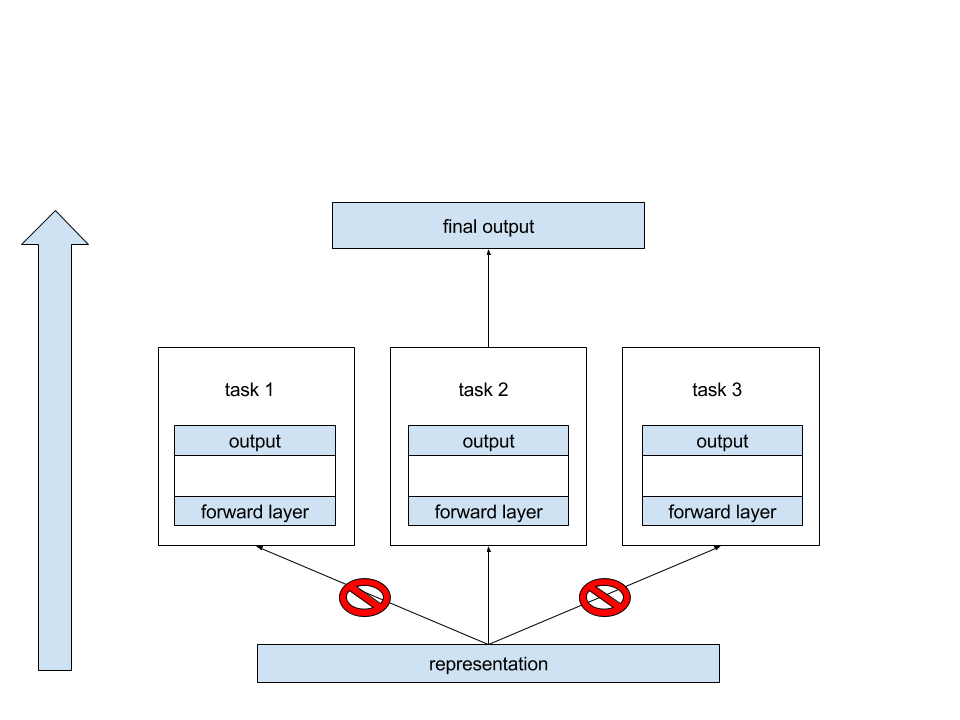
\includegraphics[scale=.2]{task_layers.png}
\caption{The task specific layers, with task 2 being the active one}
\label{fig:task}
\end{figure}

For the multitask component, each task consists of a feed forward layer with a tanh activation.  Taking the softmax of the result of the forward layer gives us a probability distribution over the output for the task for the classification-based tasks.  For the regression-based tasks, we take the output of the forward layer directly as the output of the system. Figure.~\ref{fig:task} illustrates the multitask component of our model. Next, we evaluate the performance of the proposed architecture with experiments.

\section{Experimental Results and Discussion}
In this section, we detail the setup of experiments, and discuss the results.
\subsection{Data Preparation}
We use the Switchboard-1 release 2 (LDC97S62) dataset \cite{switchboard}. LDC97S62 is a collection of approximately 2,400 two-sided telephone conversations among 543 speakers (302 male, 241 female) from all areas of the United States. We generate filterbanks from this data and align them with words from the transcriptions of the conversations to form the (word, filterbank) pairs that are then fed to the input of the network. The procedure for generating of the filterbanks is as follows: 
\begin{enumerate}[(1)]
\item For each utterance in the audio file, segment it using an 8000 Hz sampling rate. Each segment is of length 0.02s with 0.01s overlap, which gives 160 samples for each segment.
\item For each segment, preemphasize it, then window it using a Hamming window.
\item Compute the power spectrum for each segment.
\item Apply a 40-point Mel filterbank with triangular filters.
\item Take the logarithm of all filterbank energies.
\end{enumerate}
After this procedure, we get $F_w \times 40$ filterbank features for each utterance in the audio, where the number of frames $F_w$ depends on the length of the audio file, but in our implementation we pad or truncate the filterbanks to fixed size $F$.

Next, we align each word in the utterance with its corresponding filterbank feature to get the word-filterbank pairs. We use a \emph{hard} alignment, which uses the aligned transcriptions from \footnote{Word alignments were generated by using the most recent release of the transcriptions and performing forced alignments using ISIP's Hub 5E recognition system (which is also publicly available). These alignments were manually reviewed for accurate discrimination between speech and non-speech.\cite{switchboard}} to segment the filterbank data for each utterance according to the proportion of each word in the utterance. Specifically, for an utterance of length $T$ and its corresponding filterbank, we take a fraction $t/T$ of the filterbank for a word in the utterance of length $t$. This hard alignment, however, is highly inaccurate for several reasons: (1) due to the overlap in the windowing procedure, the ratio of the number of frames in the word $n$ to the total number of frames in the utterance $N$ does not equal to the ratio of the length of the word to the length of the utterance, i.e., $\frac{n}{N} \neq \frac{t}{T}$; (2) the Mel filterbank applies a nonlinear mapping to the power spectrum; (3) the time annotations in the transcripts are not accurate, and errors also occur when doing precision round up. These factors make it hard to accurately align the filterbank with its corresponding word. In order to compensate for the alignment errors, we force align the filterbank for one utterance with the words with overlap. This guarantees that no alignment error exceeds the boundary of the utterance, but we still expect large alignment errors within the utterance. 

In addition to creating word-filterbank pairs, we also have labels for speaker data, which include the following features we will use for our tasks: speaker identity, age, gender, and the dialect of English spoken. We were able to align this data with the speakers in the conversations and thus, create tuples of audio data and speaker labels.

\subsection{Training and Parameter Tuning}
The model is trained on a given input tuple by first randomly choosing a specific task.  We weight the task selection more heavily towards speech recognition, as there is greater variation in the outputs for speech recognition than the other tasks.  Only the shared component and the task-specific components of the selected task will be updated for an instance. 

We then train the network by iterating over the training set instances in random order.  For each instance, we train only against the given task.  Training was initially done using stochastic gradient descent (SGD) with an learning rate 0.001, but we also tested using Adagrad.  We trained two models, one using a two dimensional convolution over the filter banks, and one using a one dimensional convolution.  After tuning, our word embedding size is 1024.  For the one dimensional convolution, we used convolution sizes of 9 and 5, with 10 and 5 filters respectively.

Additionally, the multitask model is compared to single-task baselines where instead of connecting the shared component to multiple tasks, we simply feed the result of the shared layer to a single feedforward layer for each specific task.

\subsection{Results and Discussion}

\begin{figure}[h!]
\centering
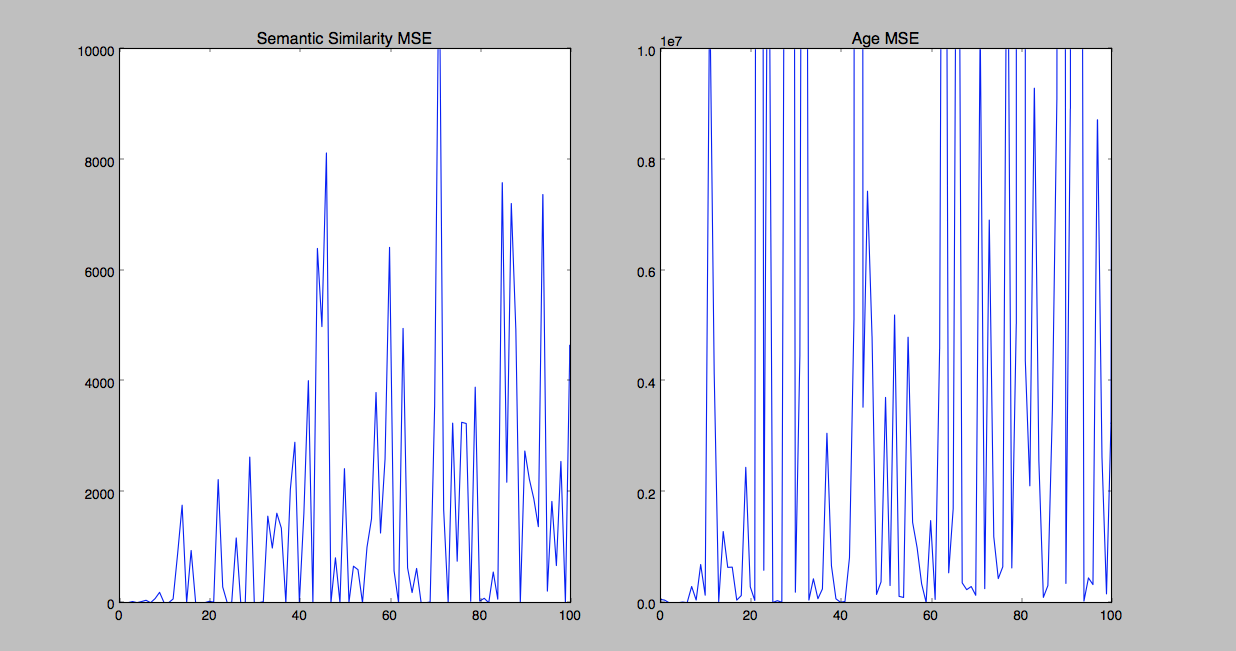
\includegraphics[scale=.2]{images/sgd_mle.png}
\caption{The MSE on semantic similarity and age on the nth dev update, trained with SGD}
\label{fig:mse_semantic_age}
\end{figure}

\begin{figure}[h!]
\centering
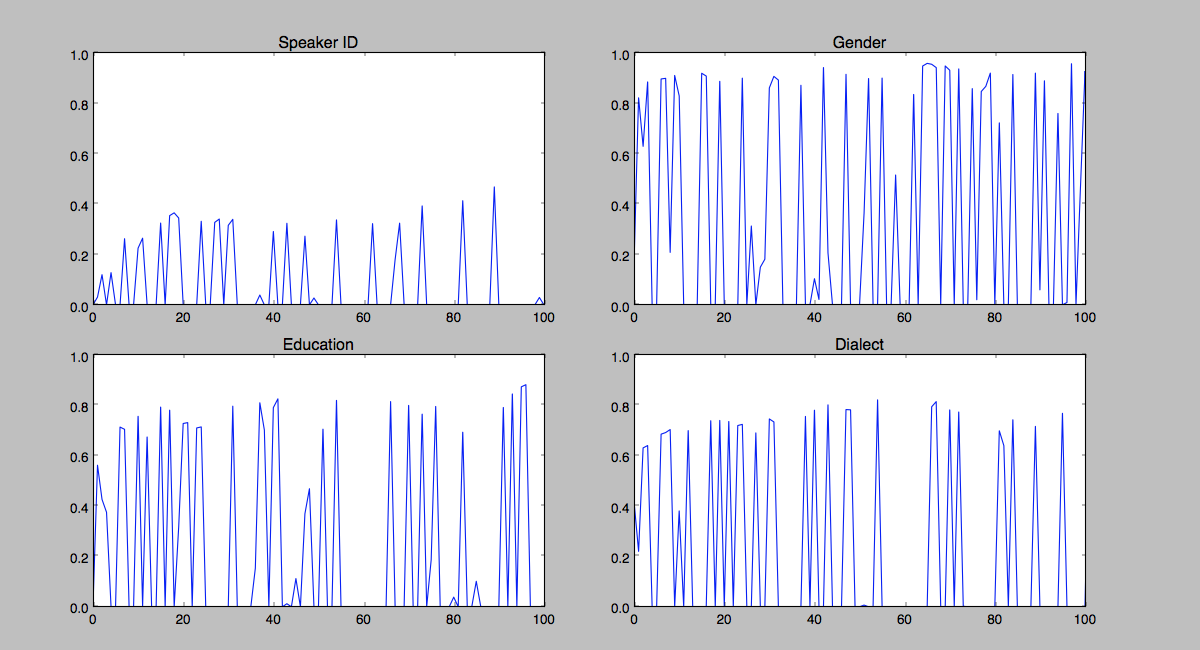
\includegraphics[scale=.25]{images/sgd_4task.png}
\caption{The probability of the correct output of the given task from the final softmax on the nth dev update, trained with SGD}
\label{fig:prob}
\end{figure}

\begin{figure}[h!]
\centering
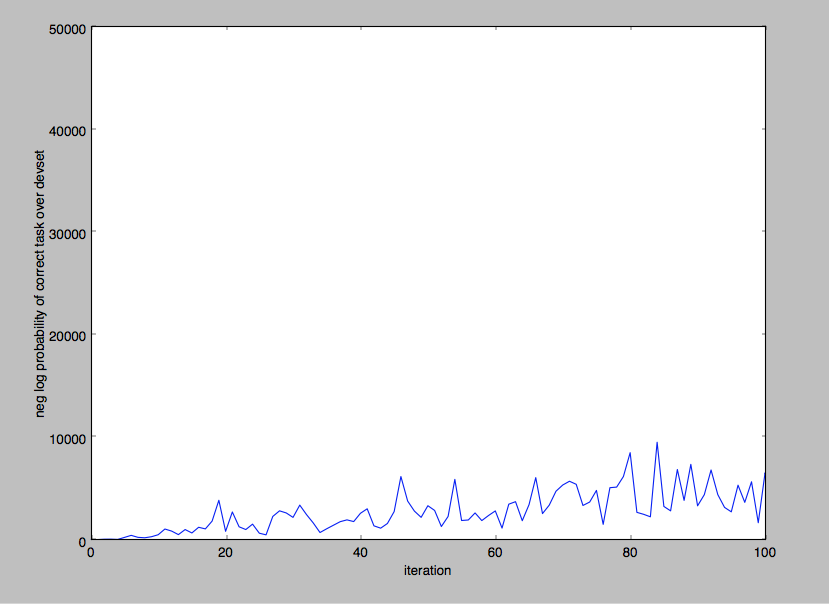
\includegraphics[scale=.2]{images/sgd_word.png}
\caption{The probability of the correct output of the word recognition task from the final softmax, trained with SGD}
\label{fig:prob_word}
\end{figure}


\begin{figure}[h!]
\centering
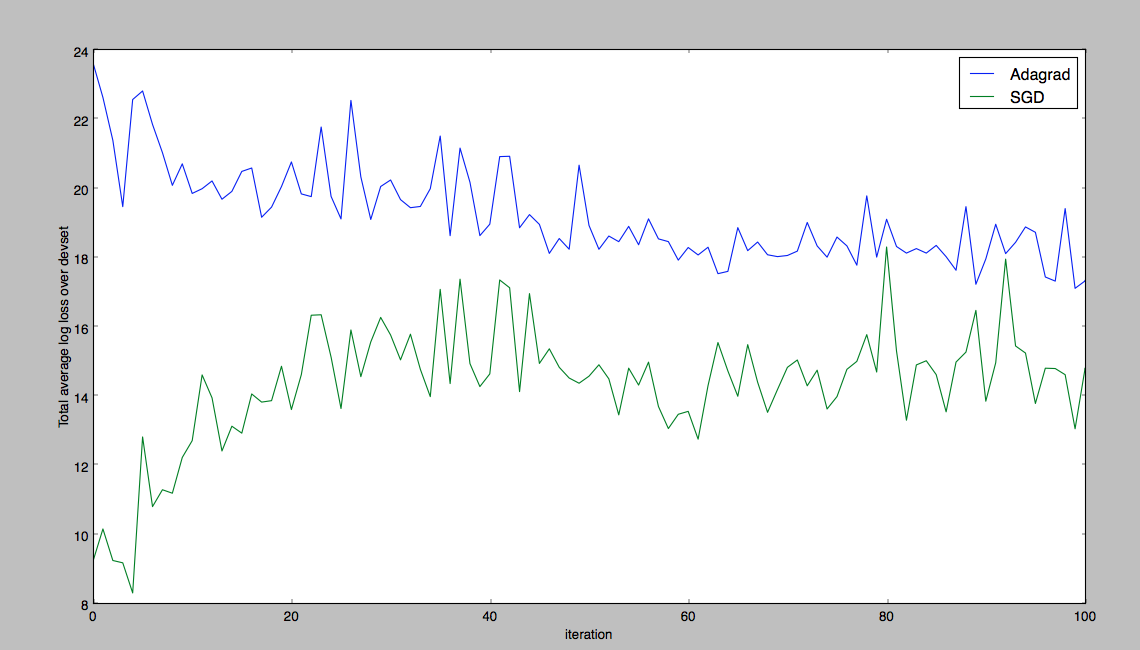
\includegraphics[scale=.2]{images/log_losses.png}
\caption{The total average log loss across the dev set for both SGD and Adagrad}
\label{fig:log_loss}
\end{figure}

When training using stochastic gradient descent (SGD), the model was not able to successfully learn multiple tasks.  As seen in Figures \ref{fig:mse_semantic_age}, \ref{fig:prob}, and \ref{fig:prob_word}, when it learns one task, the others are `forgotten', and the overall loss either increases or is at best stagnant (see Figure.~\ref{fig:log_loss}).  This is seen in the spikes in the probability of the correct answer from the final softmax and mean squared error on given tasks on a held out dev set -- when the probability of the correct answer of one task increases or the mean squared error of one task decreases, it tends to sharply increase or decrease, while the other tasks are pulled in the opposite direction.  We hypothesize that this is because as it learns one task, the other tasks are pulled away from the correct answer on those tasks.  This could be occurring because the tasks are less related than they are in text level word embeddings.  For example, in Collobert et al. \citep{collobert2008unified}, part of speech tagging and semantic role labeling are more related than age and dialect prediction, as the part of speech of a word plays a role in the meanings it can take on.  On the other hand, age and dialect are independent and can be expressed very differently in the speech signal. As a result, when training on the dialect task, the parameters are pushed towards the optimal solution for dialect identification but away from age prediction. To test this, we compared our model to a single task model with the same shared architecture on individual tasks. Table ~\ref{tab:single_task_resul} shows the results of the single-task model and we found that the network was indeed able to learn on the individual task level.  This suggests that our hypothesis is correct -- the proposed multitask model is learning the individual tasks but forgetting the other previously learned tasks.

\begin{table}[h!]
\centering
\caption{Single task results.}
\label{tab:single_task_resul}
\begin{tabular}{c|cccccc}
\hline
Task & Age & Gender & Word & Education & Dialect & Speaker \\ \hline
Error &  0.01510 & 0.02093 & 0.1592 & 0.1662 & 0.2093 & 0.2869 \\ \hline
\end{tabular}
\end{table}

To address this problem, we retrained our model using Adagrad instead of SGD as our gradient descent update rule.  As SGD updates each parameter using a constant learning rate, if the learning rate is too large, each update can push all the other tasks far enough away from the correct answer that the algorithm cannot recover.  On the other hand, Adagrad adjusts the learning rate based on the frequency of updates for a parameter, favoring smaller updates for more frequently updated parameters.  This may dampen the swings in probability we are seeing.  After training, we found Adagrad did indeed limit the spikes -- although they still occur, there were fewer and less regular wild swings in probability and MSE, while the overall error decreased (Figures ~\ref{fig:mse_semantic_ada}, \ref{fig:prob_ada}, \ref{fig:prob_word_ada}).  However, the average overall loss was higher for Adagrad compared to SGD (Figure ~\ref{fig:log_loss}).  This suggests while Adagrad does dampen the wild swings in loss, it also prevents any one task from being learned well.

\begin{figure}[h!]
\centering
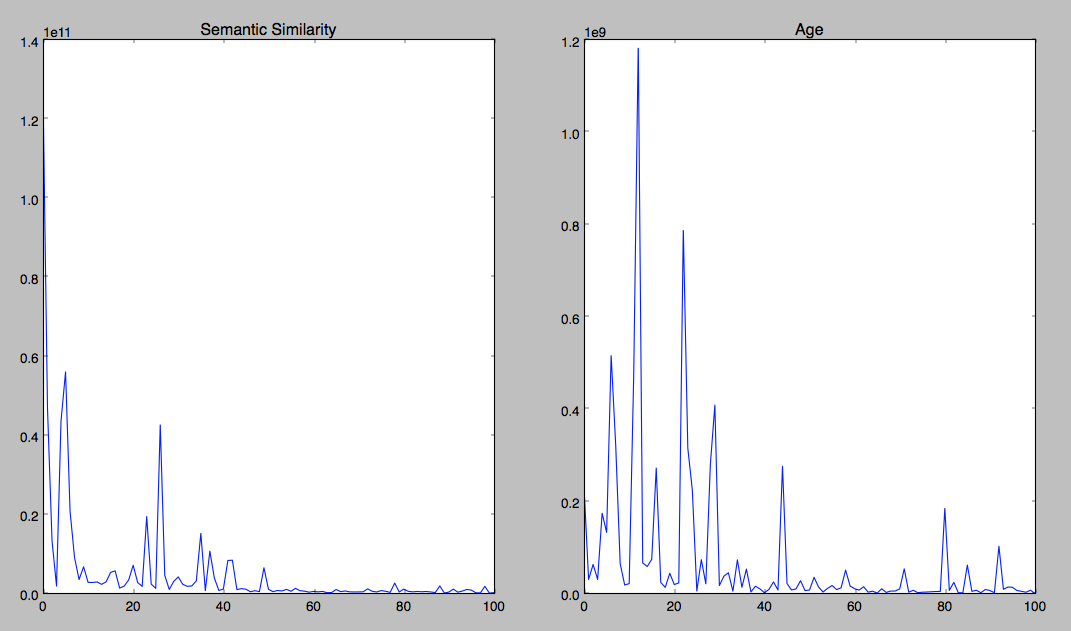
\includegraphics[scale=.2]{images/adagrad_mle.png}
\caption{The MSE on semantic similarity and age on the nth dev update, trained with Adagrad}
\label{fig:mse_semantic_ada}
\end{figure}

\begin{figure}[h!]
\centering
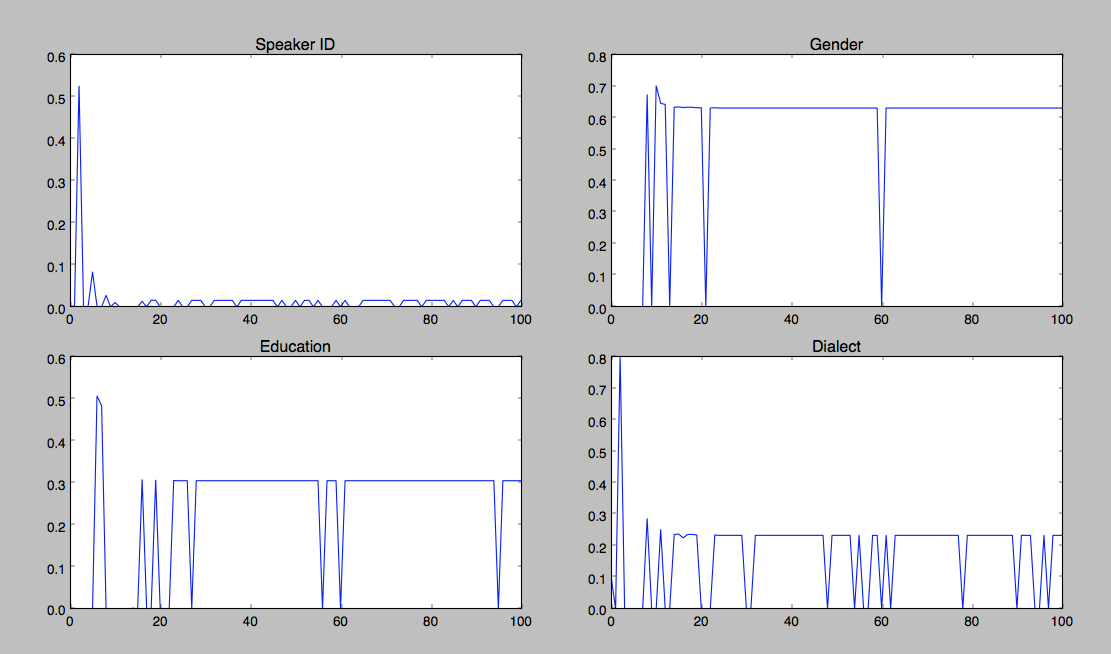
\includegraphics[scale=.25]{images/adagrad_4task_prediction.png}
\caption{The probability of the correct output of the given task from the final softmax on the nth dev update, trained with Adagrad}
\label{fig:prob_ada}
\end{figure}


\begin{figure}[h!]
\centering
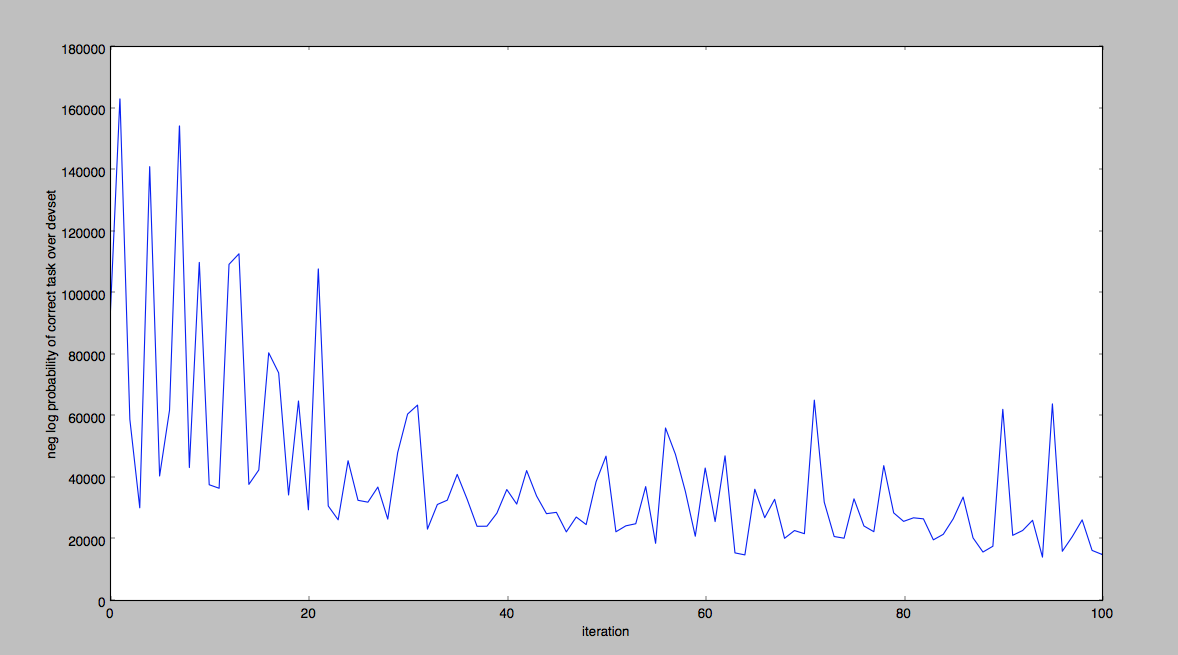
\includegraphics[scale=.2]{images/adagrad_word_prediction.png}
\caption{The probability of the correct output of the word recognition task from the final softmax, trained with Adagrad}
\label{fig:prob_word_ada}
\end{figure}

\section{Future Work}
There are a few approaches we can take to try to improve the results.  The first is to create more accurate word-filterbank alignments, as our current alignment approach returns noticeable mistakes.  We propose using well-trained acoustical model and Viterbi decoding to determine word boundaries to create more accurate word-filterbank alignments.  The second is to simultaneously train against all tasks for a given instance instead of just choosing one task for an instance and training only the task-specific components.  This would force the network to consider all of the tasks together and prevent it from focusing on the current task at the cost of all of the other tasks.  This, however, may result in similar results to Adagrad, where there are no longer drastic swings in probability and MSE, but instead the tasks are not learned all that well.  We also could try to insulate the shared representation layer by adding more layers between it and the output layer.  Using this approach, the shared representation layer would change less during training, as the intermediate layers would be able to adjust more without relying as much on the shared representation layer.

\section{Conclusions}
In this paper, we presented a multitask learning architecture creating word embeddings while capturing both acoustical and semantic information in speech signals, and found that it learned well for each individual task, but the tasks were not related enough to properly learn embeddings for accurate multitask predictions using a standard architecture.  We further found that standard gradient descent update approaches suffer from different drawbacks, and compared it with Adagrad, but neither were sufficient to make accurate multitask predictions.

\bibliography{references}
\bibliographystyle{unsrt}

\end{document}